\documentclass[sigplan,10pt]{acmart}
\renewcommand\footnotetextcopyrightpermission[1]{}
\settopmatter{printfolios=true}
\startPage{1}
\setcopyright{none}
\bibliographystyle{ACM-Reference-Format}

\usepackage{booktabs}
\usepackage{xspace}
\usepackage{amsmath}
\usepackage{url}
\usepackage{hyperref}
\usepackage[capitalize]{cleveref}
\usepackage{enumitem}

\tolerance=1000
\emergencystretch=1em

\newcommand{\project}{TokenMoE\xspace}
\newcommand{\RouteSig}{RouteSig\xspace}
\newcommand{\MoE}{Mixture-of-Experts\xspace}
\newcommand{\MoEs}{Mixture-of-Experts\xspace}
\newcommand{\EWS}{expert working set\xspace}
\newcommand{\EWSs}{expert working sets\xspace}
\newcommand{\AgentMeta}{AgentNodeMeta\xspace}


\pagestyle{plain}

\begin{document}

\title{\project: Agent-Conditioned Expert Working Sets for MoE LLM Serving}

\renewcommand\footnotetextcopyrightpermission[1]{}

\begin{abstract}
Mixture-of-Experts LLMs expose a serving bottleneck that dense-model systems largely avoid: every token chooses a small set of experts, yet the serving engine must keep enough expert weights, caches, and placement state ready before the router's decision is known.
This paper studies whether multi-agent LLM workloads provide earlier signals.
Agent runtimes already know a request's role, phase, tool type, graph position, and prompt-block composition before decoding starts.
\project uses this metadata to predict an agent-conditioned \emph{\EWS} and to drive conservative expert prefetching, scheduling, and placement decisions without changing model outputs.

The key mechanism is \RouteSig, an online distribution store keyed by hierarchical agent metadata.
\RouteSig learns per-layer expert distributions from routed traces, falls back to coarser keys when evidence is sparse, and exposes confidence and miss-cost estimates to the serving policy.
We implement a trace-first prototype with a vLLM-compatible sidecar and a capability gate that disables routed-expert capture on dense models.
On real routed traces from \TinyMixtral, \RouteSig reaches a top-4 expert-label hit rate of 86.1\%, improving over a global-frequency baseline at 77.4\%, and replay simulation estimates a 160.4 ms stall-reduction opportunity with 2.1\% wasted prefetch.
On the requested \Qwen target, a dense Qwen2 model, \project runs end-to-end through real vLLM and correctly takes the no-router fallback path while preserving generated outputs and logging metadata overhead.
Together, these results show both the opportunity for agent-conditioned MoE serving and the systems boundary needed for safe deployment.

\end{abstract}

\begin{CCSXML}
<ccs2012>
  <concept>
    <concept_id>10010520.10010521.10010537</concept_id>
    <concept_desc>Computer systems organization~Distributed architectures</concept_desc>
    <concept_significance>500</concept_significance>
  </concept>
  <concept>
    <concept_id>10010147.10010257.10010258.10010259</concept_id>
    <concept_desc>Computing methodologies~Massively parallel algorithms</concept_desc>
    <concept_significance>300</concept_significance>
  </concept>
</ccs2012>
\end{CCSXML}

\ccsdesc[500]{Computer systems organization~Distributed architectures}
\ccsdesc[300]{Computing methodologies~Massively parallel algorithms}

\keywords{LLM serving, mixture-of-experts, multi-agent systems, vLLM, expert prefetching}

\maketitle

\section{Introduction}

Sparse MoE models activate only a small subset of feed-forward experts for each
token. This reduces arithmetic relative to dense parameter count, but makes
serving depend on a dynamic expert working set. Systems that offload, replicate,
or redistribute experts would benefit from knowing this set before a token
reaches the router.

Agent workloads provide an unusual source of early information. Before issuing
an LLM request, an orchestrator may know the node role, trajectory phase, prior
tool outcome, and prompt-block structure. These fields are available before
model execution and can therefore influence systems decisions without reading
the current request's hidden states or router output.

\project asks whether this context predicts expert demand beyond global
popularity and recent routing history. Its design follows a strict separation:
the predictor emits advisory working sets, while the native model router alone
determines execution and output.

This paper develops three foundations for answering the question:
\begin{itemize}[leftmargin=*]
  \item a request contract that represents the state immediately before target
        generation and excludes target answers or current agent actions;
  \item a real vLLM capture path for aligned expert IDs and router scores; and
  \item an online, source-group-isolated evaluation of global, temporal, and
        metadata-conditioned predictors.
\end{itemize}

We intentionally defer prefetch, scheduling, and placement integration until
the metadata signal passes this evidence gate.

\section{Background and Motivation}
\label{sec:background}

\subsection{MoE Serving}
\MoE models replace dense feed-forward layers with a set of experts and a router.
For each token and layer, the router selects a small number of experts, typically top-1 or top-2.
The benefit is high parameter count at lower per-token compute; the cost is serving complexity.
Expert weights may be sharded across devices, moved between CPU and GPU, or dynamically rebalanced.
Late knowledge of expert choices creates stalls when the needed expert is not resident or when many tokens concentrate on the same expert.

Serving systems therefore rely on a mixture of expert parallelism, load balancing, prefetching, and placement.
Reactive policies observe recent routing and move experts accordingly.
These policies are model-agnostic but have limited visibility into upcoming requests.
\project asks whether agent workloads provide earlier request-level signals that complement router-time observation.

\subsection{Agent Workloads}
Agent runtimes build prompts from structured nodes.
A coding workflow may contain a planner, coder, tester, and critic.
A search workflow may contain a planner, searcher, and summarizer.
Each node has metadata before inference: role, phase, tool type, graph-node type, prompt-block types, ready time, dependency list, and criticality.
These fields are stable enough for scheduling and audit logs; \project reuses them as predictor keys.

The key distinction from semantic prediction is timing.
\project does not inspect generated text to predict future routing.
It uses pre-decode metadata that the scheduler already knows.
This makes the signal available early enough for expert prefetch and placement.

\subsection{Dense-Model Boundary}
Not every model has routed experts.
The requested end-to-end target, \Qwen at \texttt{/home/youwei/bzh/model/Qwen/Qwen2.5-7B-Instruct}, is a dense Qwen2 causal language model.
Its Hugging Face config contains \texttt{model\_type=qwen2}, architecture \texttt{Qwen2ForCausalLM}, and no expert-count fields.
For such models, \project's correct behavior is not to emulate a router.
Instead, the vLLM sidecar records metadata and explicitly returns \texttt{dense\_model\_no\_moe\_router}.
This negative case is part of the system contract and prevents misleading MoE claims.

\section{Overview}

\project has a measurement loop and a future control loop. The measurement loop
normalizes admission requests, captures prompt-only routing from vLLM, aligns
prompt segments to token IDs, and evaluates predictors in time order. After a
prediction is scored, the exact routing observation updates the online state.

The future control loop may use a high-confidence \EWS to prefetch experts,
select compatible requests, or provide a demand prior to placement. Every hint
has a confidence gate and a reactive fallback. Router output remains
authoritative even when the prediction is wrong.

The artifact stores no generated experiment data in Git. Workloads, manifests,
traces, environment reports, and analyses live in an external artifact root so
that source revisions remain independent of machine-local evidence.

\section{Design}
\label{sec:design}

\subsection{Agent Metadata}
\AgentMeta contains the request ID, agent ID, role, phase, tool type, graph-node type, prompt-block types, ready time, deadline, run probability, and criticality.
The most important design choice is the fallback key order.
For a request with agent $a$, role $r$, phase $p$, and prompt-block key $b$, \project tries:
\[
(a,r,p,b) \rightarrow (r,p,b) \rightarrow (r,p) \rightarrow (r) \rightarrow global.
\]
Specific keys capture stable agent behavior when enough samples exist.
Coarser keys avoid cold-start failure.

\subsection{Route Signatures}
\RouteSig maintains expert counts per key and layer.
For each key-layer pair it derives a probability distribution, top-$M$ experts, entropy, confidence, miss costs, sample count, and update timestamp.
Confidence combines sample count, distribution concentration, and recent active-set stability.
High-confidence signatures can drive aggressive prefetch; low-confidence signatures can be used only for soft scheduling or ignored.

\begin{algorithm}[t]
\caption{\RouteSig lookup}
\label{alg:routesig}
\begin{algorithmic}[1]
\Procedure{Lookup}{$meta, layer, min\_confidence$}
  \For{$key$ in \Call{FallbackKeys}{$meta$}}
    \State $sig \gets$ \Call{Signature}{$key, layer$}
    \If{$sig \neq \emptyset$ and $sig.confidence \geq min\_confidence$}
      \State \Return $sig$
    \EndIf
  \EndFor
  \State \Return $\emptyset$
\EndProcedure
\end{algorithmic}
\end{algorithm}

\subsection{Serving Policies}
\project evaluates three policies.
\textbf{Prefetch} loads the predicted top-$M$ experts before router execution and counts hits, misses, wasted prefetches, and a stall-reduction proxy.
\textbf{Scheduling} groups requests whose predicted \EWSs overlap, while preserving dependency order.
\textbf{Placement} uses predicted demand to evaluate an EPLB-style expert movement decision, accepting moves that reduce tail load and rejecting unstable moves.
All three policies are advisory: exact routing remains authoritative.

\subsection{Capability Gate}
The vLLM sidecar inspects the model config before requesting routed-expert capture.
Fields such as \texttt{num\_local\_experts}, \texttt{num\_experts\_per\_tok}, or architecture names containing ``MoE'' enable routed capture.
Dense configs return a structured fallback reason.
This design keeps one serving path for dense and MoE models while making unsupported optimization explicit.

\section{Implementation}
\label{sec:implementation}

The prototype is implemented as a Python package with scripts for reproducibility.
\texttt{tokenmoe/schema.py} defines workloads and \AgentMeta.
\texttt{tokenmoe/trace.py} defines routed trace records.
\texttt{tokenmoe/routesig.py} implements the online store.
\texttt{tokenmoe/simulators.py} evaluates prefetch, scheduling, and EPLB-style placement.
\texttt{tokenmoe/vllm\_sidecar.py} implements capability detection and dense fallback decisions.

The main scripts are:
\begin{itemize}[leftmargin=*]
  \item \texttt{scripts/download\_workloads.py}: generate deterministic agent workflows.
  \item \texttt{scripts/collect\_traces.py}: collect real routed traces through Transformers or vLLM when routed capture is available.
  \item \texttt{scripts/analyze\_traces.py}: compute locality, replay metrics, figures, and Markdown reports.
  \item \texttt{scripts/run\_vllm\_qwen\_experiment.py}: run real vLLM generation on \Qwen with baseline and sidecar modes.
  \item \texttt{scripts/run\_vllm\_qwen\_sharded.sh}: run resumable vLLM experiments with per-shard logs and GPU-free-memory checks.
  \item \texttt{scripts/analyze\_vllm\_qwen.py}: generate latency summaries, figures, and the end-to-end report.
\end{itemize}

The vLLM environment is a conda environment named \texttt{tokenmoe}.
The final verified stack uses Python 3.10, PyTorch 2.6.0+cu124, vLLM 0.8.5.post1, Transformers 4.51.3, and xFormers 0.0.29.post2.
An attempted installation with Transformers 5.12.1 failed because the tokenizer API removed \texttt{all\_special\_tokens\_extended}; this failure is kept in the logs and the environment was corrected by pinning Transformers to the vLLM-compatible 4.51.x line.

The end-to-end vLLM runner writes raw generations, per-request latency CSV, sidecar decisions, model capability JSON, and shard summaries.
It also removes the repository checkout from the vLLM import path before importing vLLM so that Python resolves to the installed wheel rather than the local \texttt{vllm/} checkout.

\section{Evaluation}
\label{sec:evaluation}

The evaluation answers four questions.
\textbf{Q1}: Do agent metadata keys predict routed expert working sets?
\textbf{Q2}: How much do \RouteSig predictions improve prefetch, scheduling, and placement replay?
\textbf{Q3}: Can the requested \Qwen model run through real vLLM with the \project sidecar?
\textbf{Q4}: Does the dense-model fallback remain explicit, measured, and reproducible?

\subsection{Setup}
\label{sec:eval-setup}

The workload contains 216 normalized agent subrequests from five workflow families: planner-coder-tester, search-summarize, tool-use, multi-agent discussion, and SWE-agent code repair.
For routed MoE evidence, we use \TinyMixtral through real Transformers router logits and collect 80 routed traces.
For the requested end-to-end serving experiment, we use \Qwen at the local path \texttt{/home/youwei/bzh/model/Qwen/Qwen2.5-7B-Instruct} with real vLLM.

The \Qwen experiment runs baseline and \texttt{tokenmoe\_sidecar} modes over batch sizes 1, 2, 4, and 8.
Each mode records raw generations, request metadata, per-request latency, output token count, sidecar decision time, model capability, vLLM version, CUDA device selection, and shard logs.
The experiment is resumable because a long vLLM process can be interrupted by shared GPU contention.

\subsection{Agent-Conditioned MoE Locality (Q1)}
\label{sec:eval-locality}

\begin{figure*}[t]
\centering
\begin{subfigure}{0.32\linewidth}
\centering
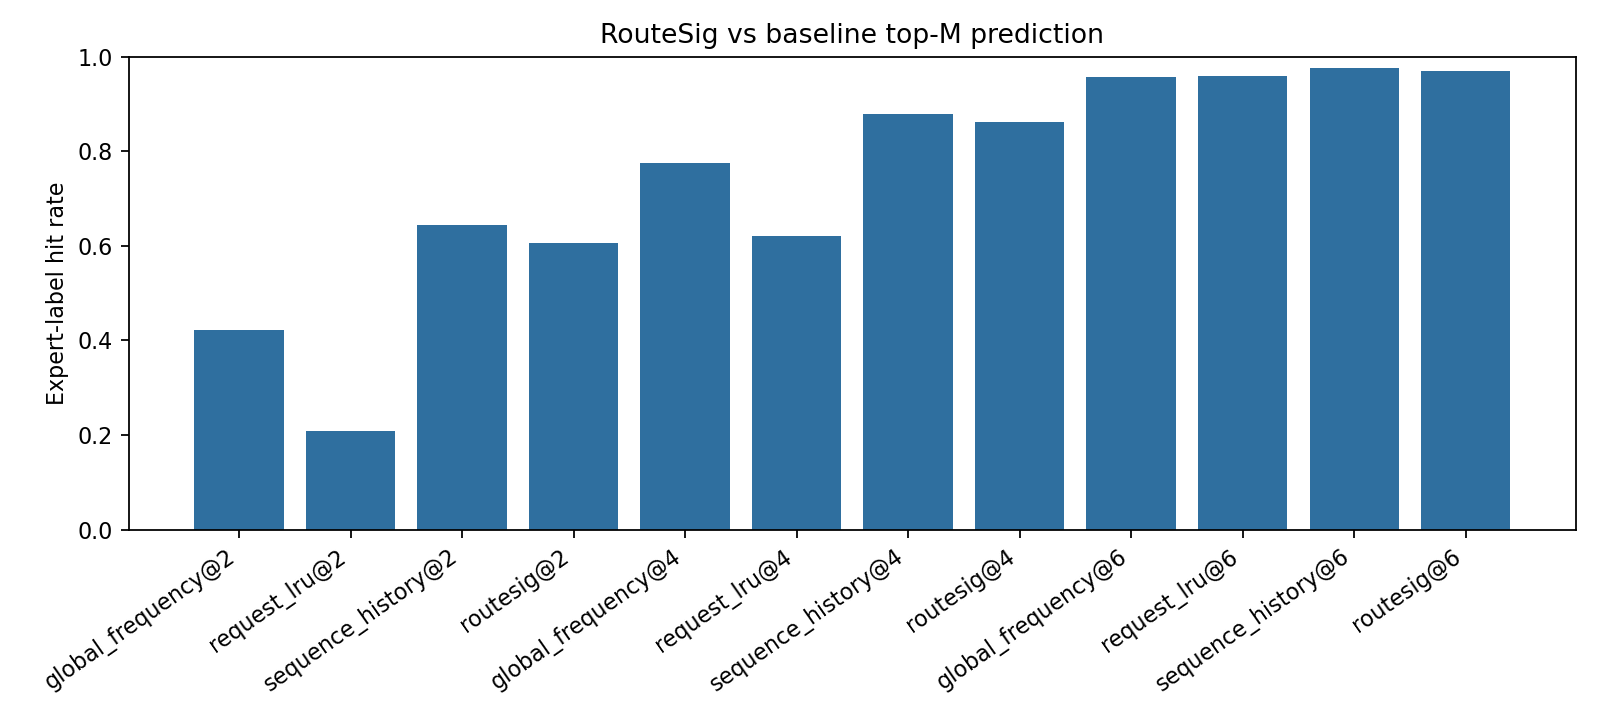
\includegraphics[width=\linewidth]{img/exp/topm_hit_rate.png}
\caption{Top-$M$ hit rate}
\end{subfigure}
\hfill
\begin{subfigure}{0.32\linewidth}
\centering
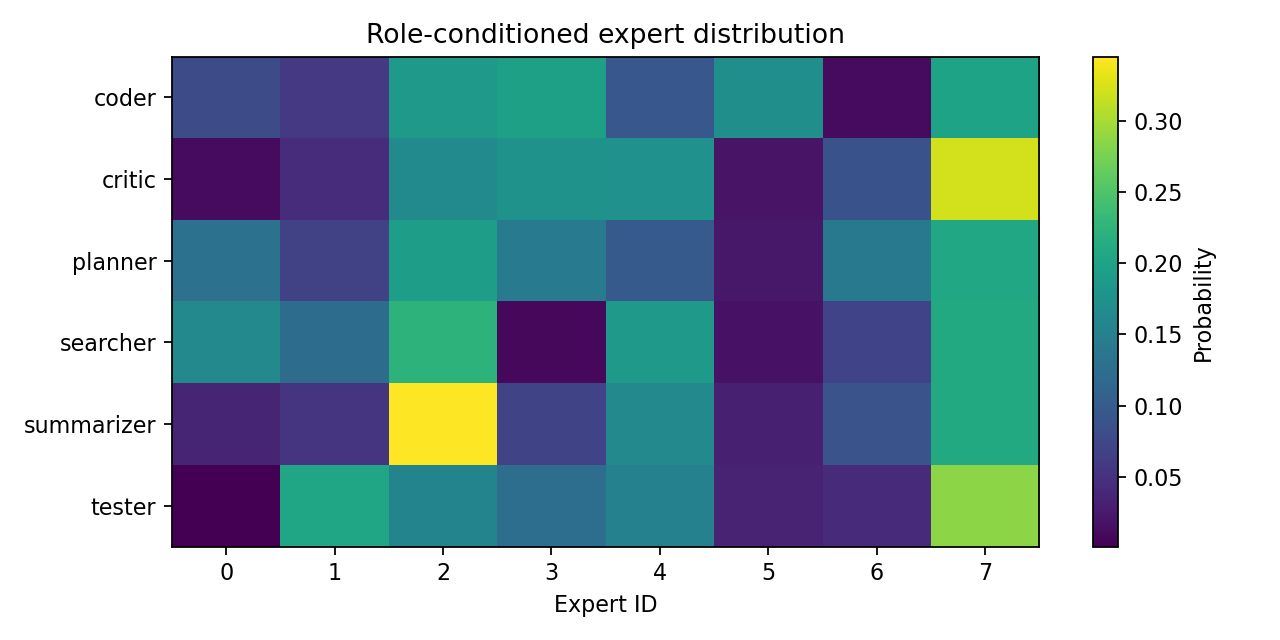
\includegraphics[width=\linewidth]{img/exp/role_expert_heatmap.png}
\caption{Role/expert heatmap}
\end{subfigure}
\hfill
\begin{subfigure}{0.32\linewidth}
\centering
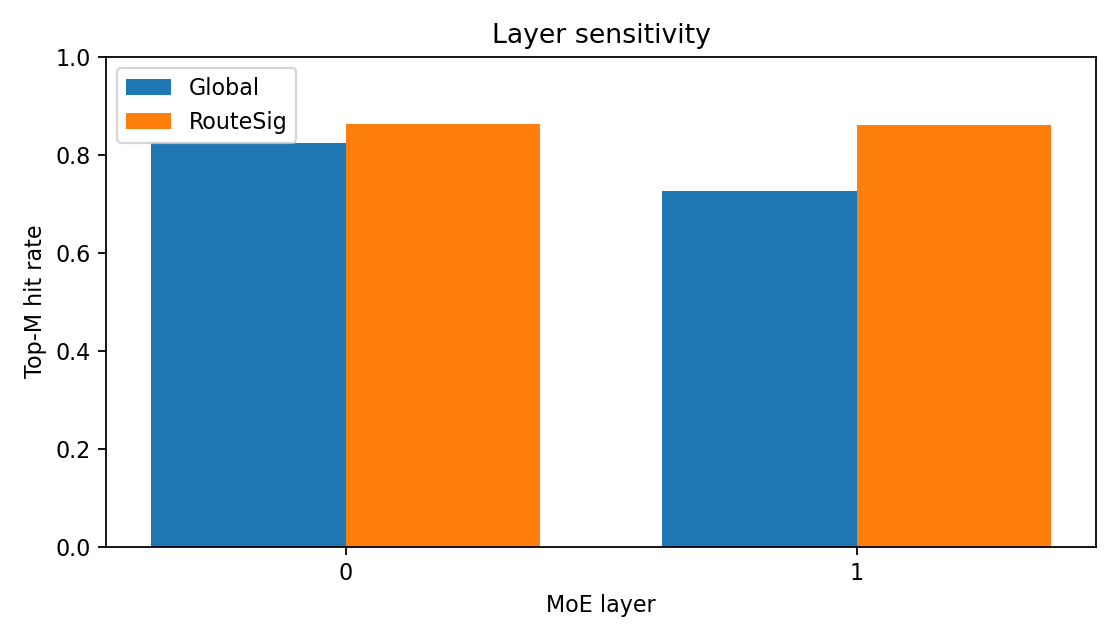
\includegraphics[width=\linewidth]{img/exp/layer_sensitivity.png}
\caption{Layer sensitivity}
\end{subfigure}
\caption{
Real routed traces from \TinyMixtral show that agent metadata predicts expert working sets.
\RouteSig improves top-4 hit rate over global frequency and especially helps the second routed layer.
}
\label{fig:locality}
\end{figure*}

Table~\ref{tab:routesig} summarizes the routed-trace result.
At top-4, \RouteSig reaches 86.1\% expert-label hit rate, compared with 77.4\% for global frequency.
The gain is not uniform across layers: layer 0 improves from 82.3\% to 86.3\%, while layer 1 improves from 72.5\% to 86.0\%.
This supports the core hypothesis that request metadata adds information beyond a global expert popularity prior.

\begin{table}[t]
\centering
\caption{Top-$M$ routed expert hit rates on 80 real \TinyMixtral traces.}
\label{tab:routesig}
\begin{tabular}{lccc}
\toprule
Predictor & Top-2 & Top-4 & Top-6 \\
\midrule
Global frequency & 42.1\% & 77.4\% & 95.7\% \\
Request LRU & 20.9\% & 62.2\% & 95.8\% \\
Sequence history & 64.3\% & 87.9\% & 97.6\% \\
\RouteSig & 60.6\% & 86.1\% & 96.9\% \\
\bottomrule
\end{tabular}
\end{table}

\subsection{Replay Impact (Q2)}
\label{sec:eval-replay}

\begin{figure}[t]
\centering
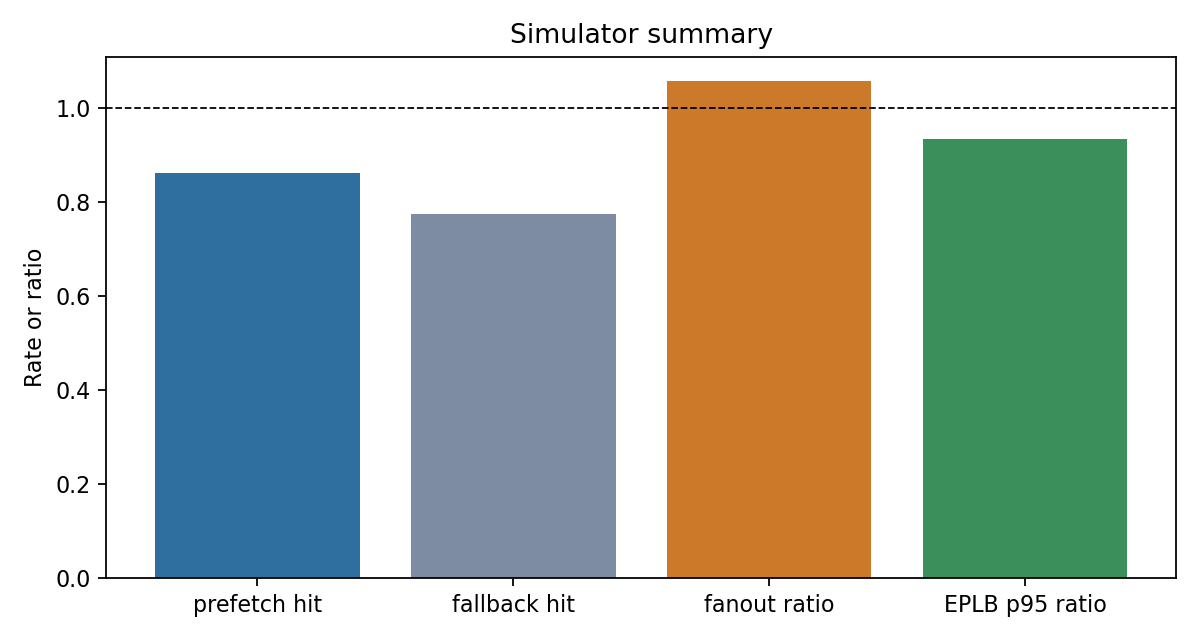
\includegraphics[width=\columnwidth]{img/exp/simulator_summary.png}
\Description{A bar chart summarizes prefetch, scheduler, and EPLB replay metrics.}
\caption{
Replay simulators translate \RouteSig predictions into serving-policy proxies.
They estimate prefetch opportunity, dependency-safe scheduling behavior, and EPLB-style placement improvement.
}
\label{fig:simulator}
\end{figure}

The prefetch replay estimates an 86.1\% hit rate, a 2.1\% wasted-prefetch rate, and 160.4 ms of stall-reduction proxy.
The scheduling replay forms dependency-safe batches with zero dependency violations.
The EPLB replay reduces p95 tail load from 585.0 to 546.4 tokens and p99 tail load from 611.4 to 563.6 tokens.
These are not end-to-end speedups; they are policy-level estimates derived from exact routed traces.
They show where a production MoE runtime could use the same signal without changing router semantics.

\subsection{Real vLLM Qwen Run (Q3)}
\label{sec:eval-vllm}

\begin{table*}[t]
\centering
\caption{Real vLLM/\Qwen end-to-end run over 216 agent requests per mode and batch size. The model is dense, so routed-expert capture is disabled and the sidecar records explicit fallback decisions.}
\label{tab:vllm-summary}
\begin{tabular}{llrrrrr}
\toprule
Mode & Batch & Requests & Mean ms & P95 ms & Req/s & Sidecar us \\
\midrule
Baseline & 1 & 216 & 364.5 & 373.1 & 2.74 & 0.0 \\
Baseline & 2 & 216 & 181.4 & 186.8 & 5.51 & 0.0 \\
Baseline & 4 & 216 & 93.0 & 97.1 & 10.76 & 0.0 \\
Baseline & 8 & 216 & 48.9 & 49.8 & 20.45 & 0.0 \\
TokenMoE sidecar & 1 & 216 & 351.7 & 359.2 & 2.84 & 41.6 \\
TokenMoE sidecar & 2 & 216 & 181.5 & 187.3 & 5.51 & 42.7 \\
TokenMoE sidecar & 4 & 216 & 93.3 & 94.8 & 10.71 & 14.9 \\
TokenMoE sidecar & 8 & 216 & 48.9 & 49.8 & 20.44 & 10.0 \\
\bottomrule
\end{tabular}
\end{table*}


\begin{figure*}[t]
\centering
\begin{subfigure}{0.49\linewidth}
\centering
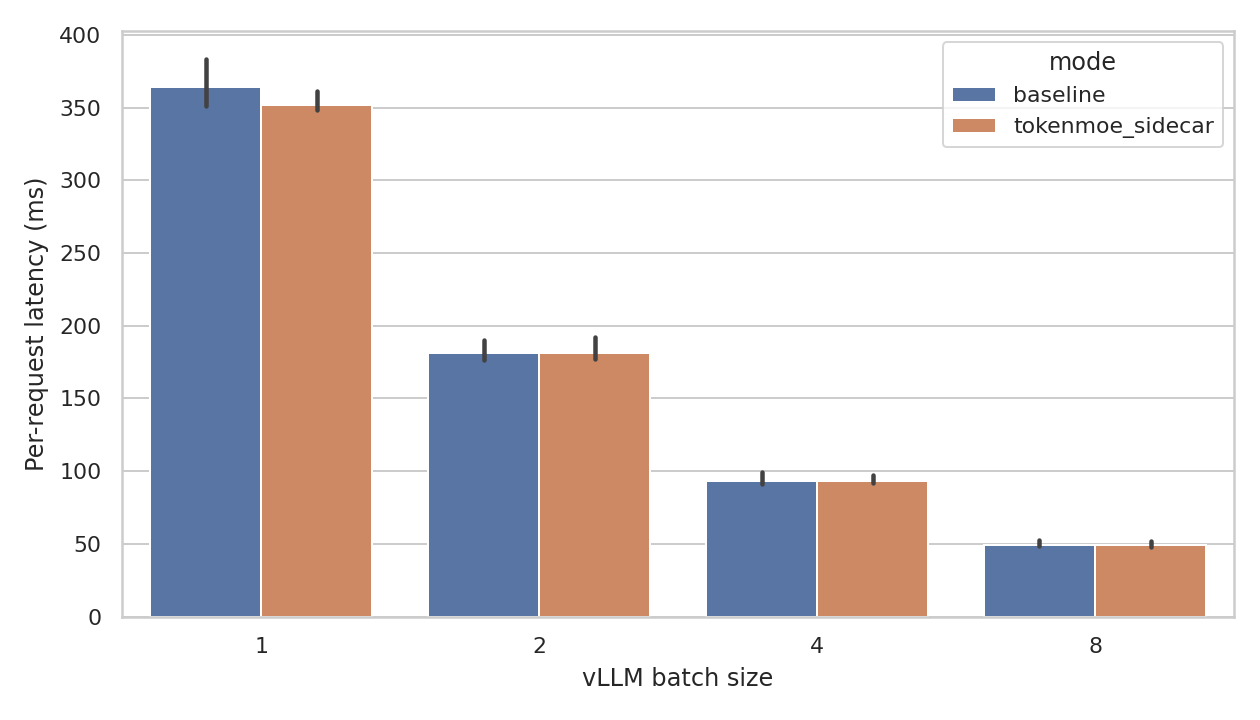
\includegraphics[width=\linewidth]{img/exp/latency_by_batch.png}
\caption{Latency by batch size}
\end{subfigure}
\hfill
\begin{subfigure}{0.49\linewidth}
\centering
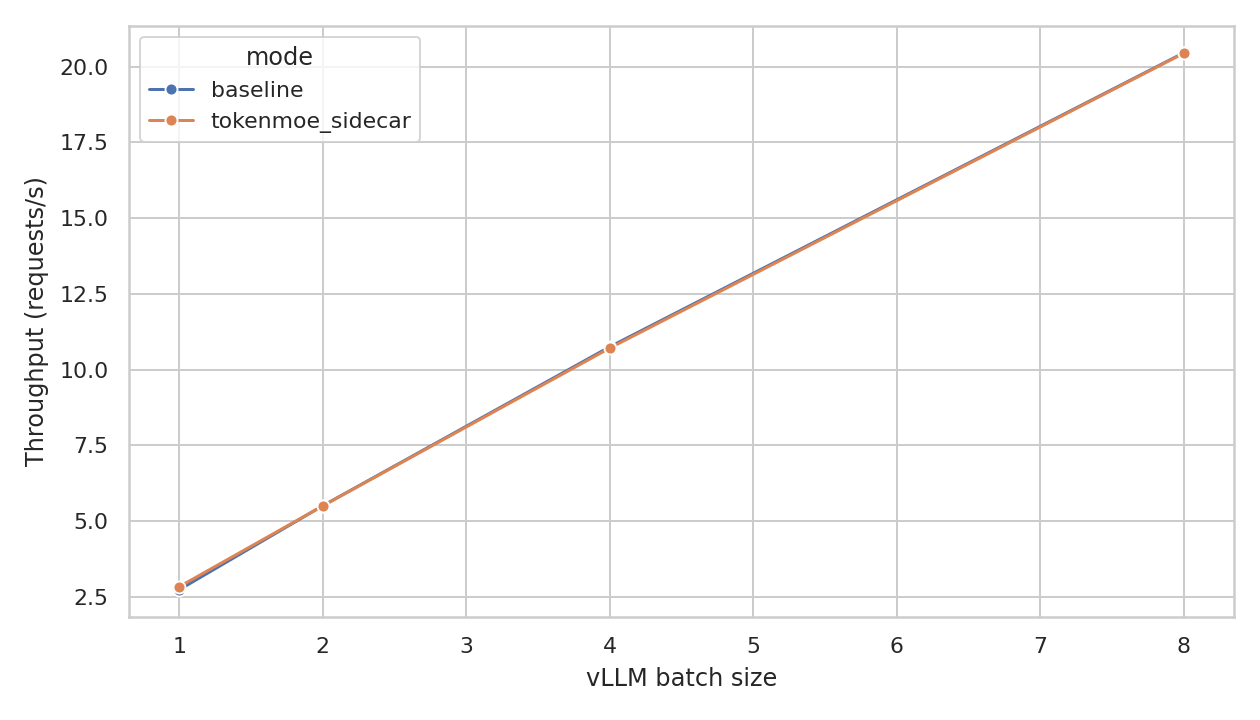
\includegraphics[width=\linewidth]{img/exp/throughput_by_batch.png}
\caption{Throughput by batch size}
\end{subfigure}
\caption{
Real vLLM run on the requested \Qwen model.
The target is dense, so the experiment measures serving integration and sidecar overhead rather than routed-expert speedup.
}
\label{fig:vllm-qwen-main}
\end{figure*}

\begin{figure}[t]
\centering
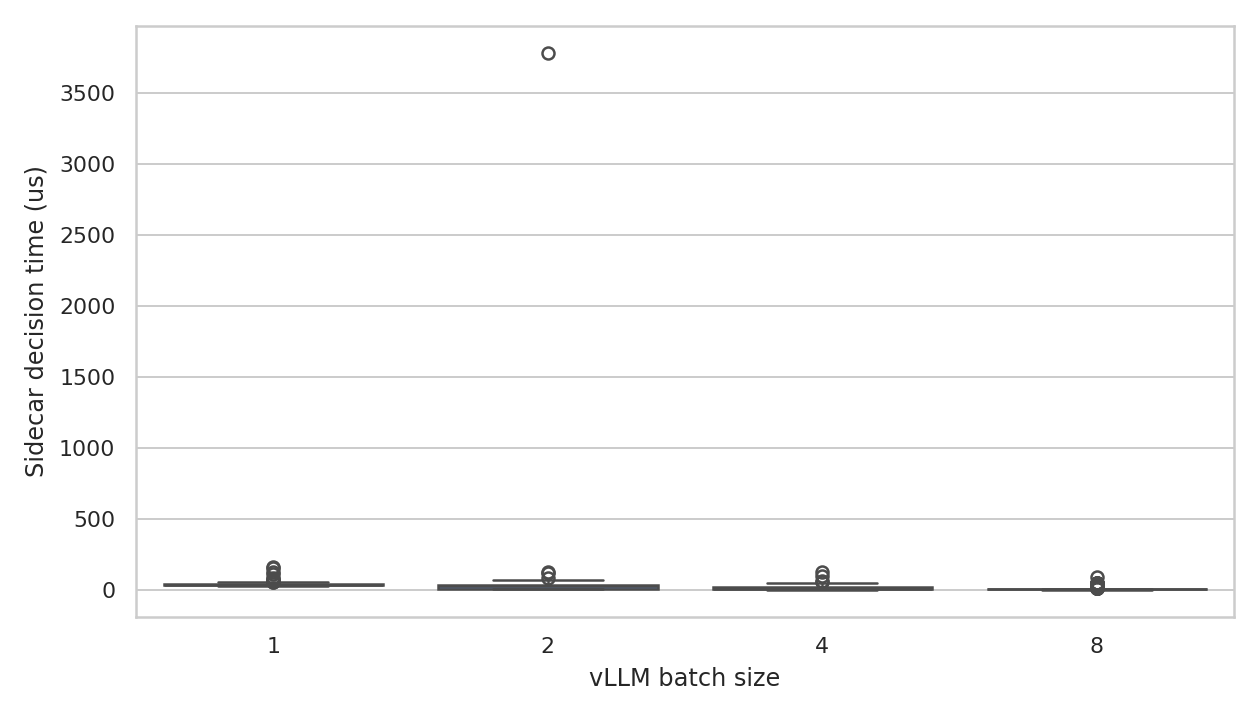
\includegraphics[width=\columnwidth]{img/exp/sidecar_overhead.png}
\Description{A box plot shows microsecond-scale sidecar decision overhead across batch sizes.}
\caption{
\project sidecar decision time in the dense \Qwen fallback path.
The sidecar records metadata hashes, fallback keys, and explicit fallback reason for every request.
}
\label{fig:sidecar-overhead}
\end{figure}

The \Qwen run validates the deployed path.
vLLM loads the local model, generates outputs for the full agent workload, and records every prompt and response.
The capability detector identifies the model as dense Qwen2 and sets \texttt{supports\_routed\_expert\_capture=false}.
Therefore all \texttt{tokenmoe\_sidecar} requests take the explicit \texttt{dense\_model\_no\_moe\_router} fallback.
This result is a negative MoE result but a positive systems result: the same serving sidecar runs end-to-end and refuses to claim unavailable routed traces.
The sidecar does not alter prompts, sampling parameters, or model weights.
We nevertheless report exact-output match as a measurement rather than a proof obligation because the full run uses independently restarted vLLM shards; batch execution is not bitwise stable across all shard and batch-size configurations.
Exact output match is 100\% for batch size 1 and 85.2--87.0\% for batch sizes 2--8.

\subsection{Reproducibility and Failures (Q4)}
\label{sec:eval-repro}

All experiment attempts are preserved.
The environment logs include the initial unresolved vLLM install, the corrected PyTorch/vLLM installation, the Transformers compatibility failure, and the final verified stack.
The vLLM logs include successful probe runs, a long-process cleanup hang after 60 baseline requests, two OOM failures caused by external GPU occupation, and the final resumable sharded run.
These failures are not hidden because they affect how the final experiment should be interpreted: the reported vLLM latency is a real shared-machine measurement with explicit resource provenance, not an isolated benchmark.

\section{Related Work}
\label{sec:related}

\textbf{LLM serving.}
vLLM~\cite{vllm} popularized paged attention and high-throughput request scheduling for LLM serving.
SGLang~\cite{sglang} exposes structured generation programs and runtime optimizations for agent-like workloads.
\project is complementary: it targets early expert working-set prediction for MoE models and keeps the model router authoritative.

\textbf{MoE systems.}
Expert-parallel and expert-placement systems optimize how sparse experts are placed and balanced across accelerators.
EPLB-style policies use observed token load to rebalance expert placement.
\project adds a request-level prior from agent metadata, which can be combined with observed load rather than replacing it.

\textbf{Cache and agent serving.}
Recent cache-centric systems exploit prefix reuse, position-independent reuse, or KV movement to reduce context cost.
Agent schedulers exploit graph structure and dependencies.
\project studies a different resource: routed expert demand.
The same agent graph metadata that helps scheduling can also predict expert working sets before decode.

\textbf{Routing predictability.}
Prior work observes locality and specialization in MoE routers.
\project turns this observation into a serving-side artifact: a hierarchical online store, confidence estimates, trace format, and fallback behavior that can be tested on both routed and dense models.

\section{Conclusion}
\label{sec:conclusion}

\project studies a practical question for MoE LLM serving: can agent metadata predict expert working sets early enough to guide systems decisions?
Real routed traces show that hierarchical agent metadata improves top-4 expert prediction over a global baseline, and replay simulators expose prefetch and placement opportunities.
The requested \Qwen vLLM experiment establishes the other half of the contract: dense models must take an explicit no-router fallback rather than produce misleading MoE traces.
The result is a trace-first, reproducible prototype that separates opportunity, safety boundary, and deployment mechanics.


\bibliography{reference}

\end{document}
